\chapter{Web application}

 In this chapter, the web application implemented as a part of this project is presented. Aspects such as the implementation and technologies used are described and the design of the user interface along with the use of the application are discussed. Finally, the evaluation and testing approaches are reported.
 
\section{Architecture and technologies used}
To be able to show the results of the experiment and allow for real time predictions of songs on Spotify a web application was implemented. It allows a user to search for a song on Spotify and see the prediction outcomes of different models. One other feature it has is the model list includes a Multi-layer Perceptron that learns after each prediction so it will improve its performance over time and it should adapt to changing trends.

The popular and unpopular labels, portrayed through the fire and the blue face emoji respectively, express whether the song's features are similar to the features of hit songs or not - if the song has the potential to be popular or not.

Having implemented the models using sci-kit learn with the selected features and optimised parameters, I have used the pickle library \cite{PickleOnline:online} that allows for object serialisation and de-serialisation to save the models to files. I then built a Flask (a Python microframework for web applications) \cite{FlaskOnline:online} back-end and a front end in HTML with Bootstrap and CSS. The user interface is responsive and works on both desktop and mobile. The way the back-end works is: on startup, the back-end loads the models from the files. When a query is sent, it gets the information for a song using the same spotipy library to interface with the Spotify API, applies the machine learning algorithm to that song and returns the resulting prediction to the user where it is displayed using the emoji labels. 

This is the case for all the classifiers except the MLP online one which does some additional operations. After it wrongly predicts a song (the output label is checked against the actual popularity value on Spotify) it will treat that song as a new learning example. In this way, its predictions will improve after each mistake so they adapt to changing trends in music.

\begin{figure}[h]
    \centering
        \centering
        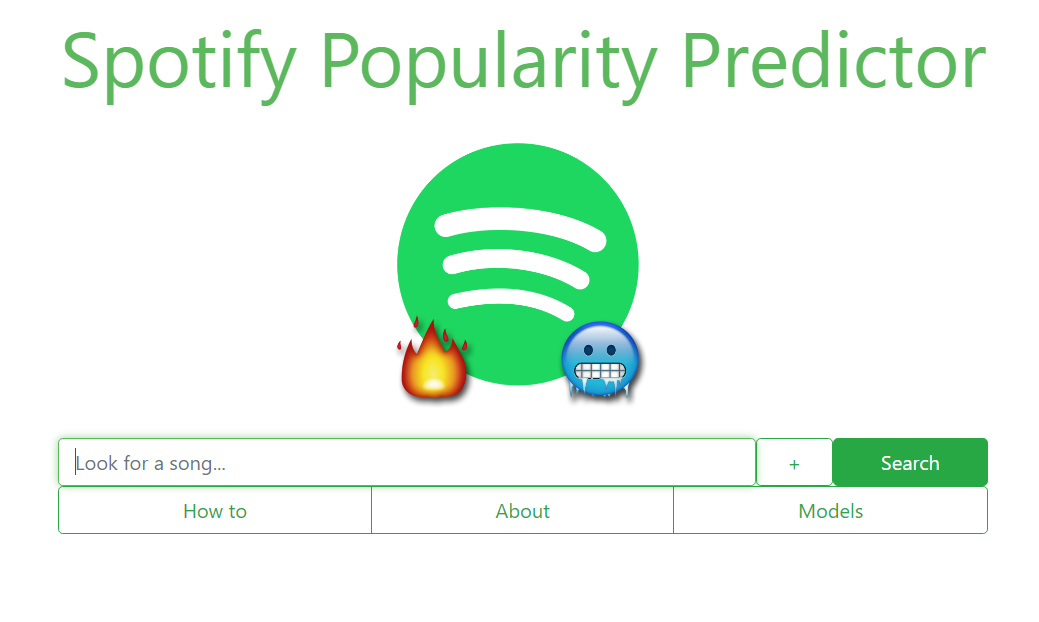
\includegraphics[width=0.8\textwidth]{web_application/fig/ui1.PNG} % first figure itself
        \caption{Landing page}
        \label{fig:ui1}
\end{figure}

% Fix to move content to the next page
% \vspace{40pt}

\begin{figure}[h]
\centering
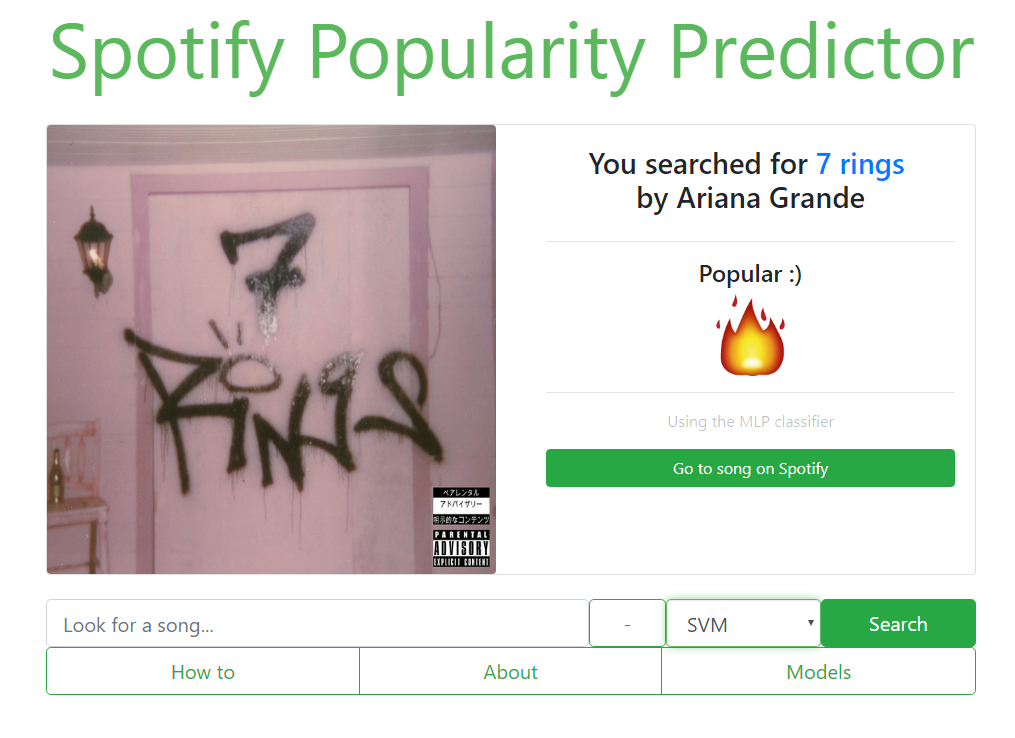
\includegraphics[width=0.8\textwidth]{web_application/fig/ui2.PNG} % second figure itself
\caption{The search performed page for the song "7 rings" by Ariana Grande}
\label{fig:ui2}
\end{figure}

This application is deployed on a cloud platform for Python and is available online \cite{WebApp:online}. It can potentially be used by artists, music labels or the media to see if a song has the characteristics of a hit song, as soon as it is posted on Spotify.

\section{Evaluation}
For the testing of the application different techniques were employed. First, the Audits available in the Google Chrome browser were used to test whether the code respects best practices relating to coding, performance, accessibility and even SEO (Search Engine Optimisation). The report can be seen in Figure \ref{fig:audit1}. The lower score in the Best Practices section relates to the fact that the application does not use the more secure HTTPS which can easily be fixed if it is required. To further ensure code quality, an online HTML validator was used.

The next step was to test the user interface and user experience design. I wanted the user interface to be as minimalistic and consistent as possible, in the same colour theme as the Spotify application and to only allow for simple, obvious interactions. By performing some tests on users such as my supervisor and several friends, some areas of possible improvement became apparent. In an early version of the application, the tabs below the search bar in Figure \ref{fig:ui1} were not implemented so a new user would have no idea what the application does, how to use it and what the results mean. Initially the selection drop-down visible in Figure \ref{fig:ui2} was not hidden so it complicated the interaction of an average user. The design was also changed to include a logo, a bigger title and a horizontal layout in the results page on desktop.

\begin{figure}[h]
\centering
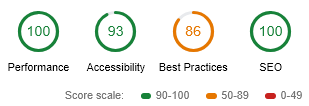
\includegraphics[width=0.6\textwidth]{web_application/fig/audit1.PNG} % second figure itself
\caption{Audit results generated in Google Chrome}
\label{fig:audit1}
\end{figure}

Since the application allows for user input, it is important to test its security even though no sensitive data is stored. Invalid queries are being displayed back to the user but the content is HTML encoded. Also, the Spotify API is used to process those queries so as long as it is secure, the application will also be, so things like database injection techniques will not work because they already have their own safeguards in place. Custom pages for invalid request, page not found, internal server error for the application have also been implemented.

To test the resilience of the application to multiple user interactions, an open source load testing tool \cite{LocustTest:online} was used that allowed the simulation of many simultaneous users. With 100 concurrent users and about 10 requests per second the application performed very well with an average response time of 760 milliseconds across the two main pages and no failures or exceptions. After 200 users some failures started to appear because of the limitations of the web host since the one being used is free but since it is cloud based with an upgrade it could scale for the demand. At 1000 users the failure rate was high but for the same reason as before. Results for the 100 and 200 user cases can be seen in Tables \ref{tab:loadtest1} and \ref{tab:loadtest2}. 


\begin{longtable}{|p{1cm}|p{2cm}|p{1.5cm}|p{1cm}|p{1cm}|p{1cm}|p{1cm}|p{1cm}|}
\hline
\textbf{Met-hod} & \textbf{Name}              & \textbf{\# req.} & \textbf{\# failures} & \textbf{Avg. resp. time} & \textbf{Min resp. time} & \textbf{Max resp. time} & \textbf{Req. /s} \\ \hline
GET             & /                          & 531                  & 0                    & 708                            & 122                        & 7368                       & 5.17                \\ \hline
GET             & /search  & 486                  & 0                    & 817                            & 225                        & 7414                       & 4.73                \\ \hline
                & Total                      & 1017                 & 0                    & 760                            & 122                        & 7414                       & 9.90                \\ \hline
\caption{Statistics of load test for 100 users}
\label{tab:loadtest1}
\end{longtable}

\begin{longtable}{|p{1cm}|p{2cm}|p{1.5cm}|p{1cm}|p{1cm}|p{1cm}|p{1cm}|p{1cm}|}
\hline
\textbf{Met-hod} & \textbf{Name} & \textbf{\# req.} & \textbf{\# failures} & \textbf{Avg. resp. time} & \textbf{Min resp. time} & \textbf{Max resp. time} & \textbf{Req. /s} \\ \hline
GET             & /             & 501                  & 32                   & 6080                     & 120                     & 11739                   & 5.49             \\ \hline
GET             & /search       & 519                  & 23                   & 6519                     & 119                     & 12062                   & 5.69             \\ \hline
                & Total         & 1020                 & 55                   & 6303                     & 119                     & 12062                   & 11.18            \\ \hline
\caption{Statistics of load test for 200 users}
\label{tab:loadtest2}
\end{longtable}

To evaluate the actual prediction results of the web application I started by searching for the top songs on the Spotify charts. Such a query can be seen in Figure \ref{fig:ui2}. That song has been very popular with over 500 million plays on Spotify and the application correctly labels it as popular, therefore the machine learning algorithm correctly identifies the pattern of popular songs in this example and the prediction is what we expect. Also, this particular song is a good example because when the data was sampled, that song had not been yet released. If the application had been used to predict the song upon its release it would have been correct in its prediction. Looking at the most played songs on Spotify from 2013 to present \cite{SpotifyCharts:online}, the application predicts 7 out of the first 10 as popular using the SVM model. 

\begin{figure}[h]
\centering
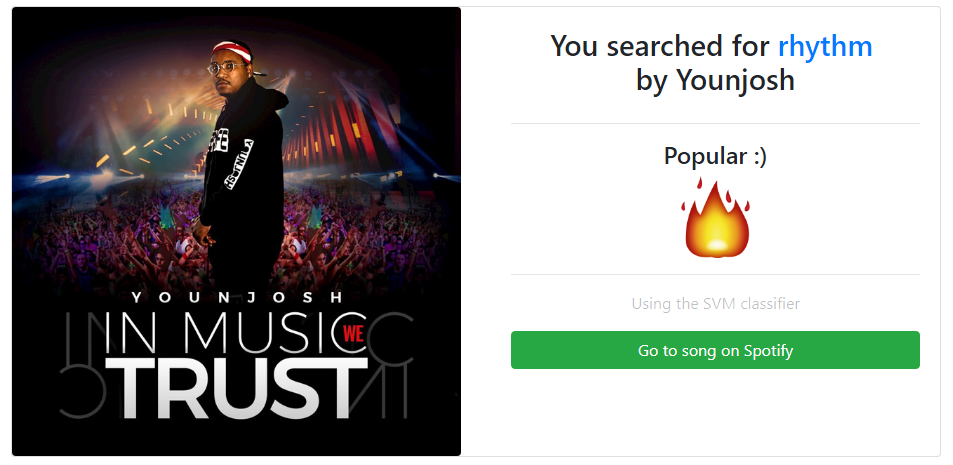
\includegraphics[width=0.7\textwidth]{web_application/fig/ui3.PNG} % second figure itself
\caption{The search performed page for the song "rhythm" by Younjosh}
\label{fig:ui3}
\end{figure}

The next step was to look for some unpopular songs to see if the application can be used to find diamonds in the rough. With less than 1000 plays, the song in Figure \ref{fig:ui3} is clearly not a hit but it was predicted as popular. Hopefully, this song might appear in the charts soon. Interestingly, it uses fragments from an older popular song from the 90's. That result means that the song has features that other hit songs present from an acoustic point of view but maybe other aspects such as the fact that the artist is unknown and lack of promotion come into play so it has not yet become a hit but the algorithm can't consider such aspects. In an ideal world where every piece of music would get the same level of exposure maybe this song could have shined through because of its hit-like features.

The algorithms do sometimes make mistakes so songs get predicted as not popular even though they might be. When this happens I noticed the songs are quite different, maybe unique in some way. The song in Figure \ref{fig:ui4} is a good example, currently being number 1 on the Spotify charts with around 5 million daily plays but it is predicted as not popular. However, the artist is currently very popular and her music is known for being different and unique so again there might be aspects that do not depend on the audio that have contributed to the popularity of this song.

Through testing the application with a lot of different songs, it looks like the performance obtained during the training and testing phase does still apply to the real world. However, to truly see if the application can indeed predict a hit, songs need to be predicted as soon as they are released and their journey followed to see if they do become popular or not which would tell us how reliable those predictions are. To prove the effectiveness of the application this would need to be done for a large number of songs to see how many of the songs predicted as popular upon their release did actually end up popular. This is not that trivial but could be done in the future.



\begin{figure}[h]
\centering
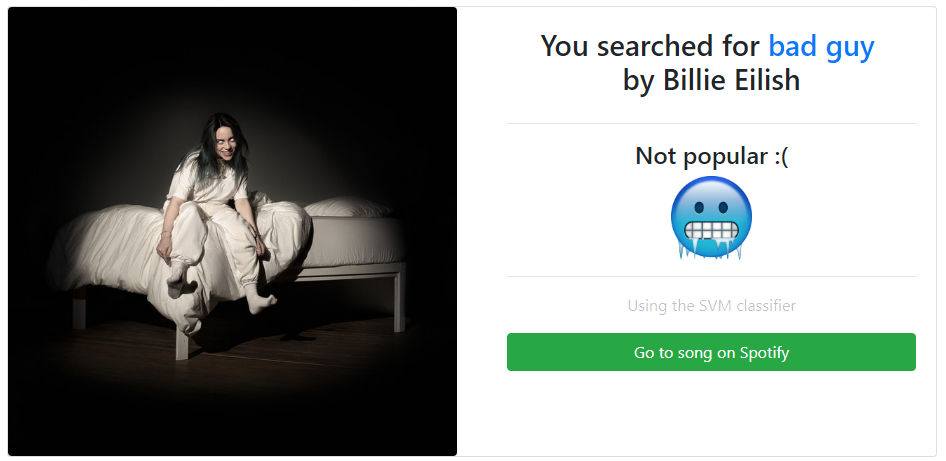
\includegraphics[width=0.7\textwidth]{web_application/fig/ui5.PNG} % second figure itself
\caption{The search performed page for the song "bad guy" by Billie Eilish}
\label{fig:ui4}
\end{figure}